\documentclass[output=paper]{langsci/langscibook}
\ChapterDOI{10.5281/zenodo.3972872}

\author{David Adger\affiliation{Queen Mary University of London}}
\title{Rethinking the syntax of nominal predication}

% \chapterDOI{} %will be filled in at production

\abstract{Human languages often disallow bare nominals as predicates. Scottish
    Gaelic is a particularly striking case, in that it disallows simple nominal
    predication entirely, using alternative syntactic means to deliver the
    required meanings. This paper provides an answer both to  the larger
    question of why NP predication is so restricted, and to the more local one
    of why Gaelic uses the particular syntactic forms it does, based on a
    principle that regulates the interface between syntax and semantics:
syntactic predicates must have open eventuality variables.}

\maketitle

\begin{document}\glsresetall

\section{Introduction}

Scottish Gaelic, like \ili{Irish}, does not allow simple noun phrase \isi{predication}, of
the type one sees in English.

\ea
\ea Lilly is a cat.
\ex Anson is a teacher.
\z
\z
This paper finds the reason for this at the interface between syntax and
semantics. I propose a general principle regulating \isi{predication} as follows:

\ea For an XP to act as a syntactic predicate, it must have a semantically open
eventuality variable.
\z

I combine this with the proposal, motivated in \textcite{adgerbook}, that
underived nouns are sortal (one place) semantic predicates of individuals, and
so never involve an eventuality variable. It follows that an NP can never act
as a syntactic predicate.

Languages, however, need to express nominal \isi{predication}, so they get around the
strictures imposed by these principles in various ways. I show how Scottish
Gaelic uses two distinct strategies for this purpose.  The overall conclusion
is that universal restrictions at the syntax semantics interface nevertheless
leave languages open to a range of syntactic solutions to express thought,
leading to restricted variability in how \isi{predication} is syntactically
expressed.

\section{The basic set of puzzles}

Languages often go out of their way to do something strange when they use
projections of nominals as predicates. For example, \ili{Scottish Gaelic} (and
related \ili{Celtic} languages), allow simple [DP predicate] orders after the finite
auxiliary when the predicate is an adjective or a prepositional phrase
(\citealt{chung-mccloskey:87}):

\ea \ili{Scottish Gaelic}\\
\gll Tha  Calum  faiceallach.\\
Be.\Prs{}  Calum  careful\\
\glt \enquote*{Calum is (being) careful.}
\ex  \ili{Scottish Gaelic}\\
\gll Tha  Calum  anns a' bh\`uth.\\
Be.\Prs{}  Calum  in the shop \\
\glt \enquote*{Calum is in the shop.}
\z
However, as noted by \citet{adger-ramchand:03}, the predicate cannot be a
nominal:

\ea \ili{Scottish Gaelic}\\
    \gll * Tha  Calum  oileanach.\\
        {} Be.\Prs{}  Calum student \\
    \glt \hspaceThis{*} intended: `Calum is a student.'\label{Calum1}
\z
There are two ways of expressing the English translation in~\eqref{Calum1}
(\citealt{cram:83,schreiner:15}). In the first, the auxiliary
subject predicate structure is maintained,  but an apparently prepositional
element appears before the nominal (I'll term this the \textit{p-strategy}):\largerpage

\ea \ili{Scottish Gaelic}\\
\gll Tha  Calum  na  oileanach.\\
Be.\Prs{}  I  in.\Poss{}.\Tsg{}.\M{}  student \\
\glt \enquote*{Calum is a student.}
\z
The alternative is to use a clefting structure (the \textit{cleft-strategy}):\footnote{\label{icc}There is,
    in formal/archaic registers, a
    third possibility, where a bare copula\is{copulas} is used (what
    \citealt{adger-ramchand:03} call the \textit{inverted copular construction}, ICC),
    as in~\eqref{archaic}. However, for simple nominal \isi{predication} at least, this
    is vanishingly rare in normal discourse:

\begin{exe}\label{archaic}
    \exi{(i)}Scottish Gaelic\\
\gll Is cat Lilly \hfill (archaic)\\
\Cop{} cat Lilly\\
\glt \enquote*{Lilly is a cat}
\end{exe}}
\ea
\gll 'S e oileanach a th' {ann an} Calum\\
\Cop{} it student \Rel{} be.\Prs{} in Calum\\
\glt \enquote*{Calum is a student.}
\z
In both strategies, the preposition \emph{ann an}, `in' appears.\footnote{A word
on the morphology of this preposition to avoid confusion in interpreting the
glosses. The bare form of the preposition used before indefinite NPs and proper
names is written as two words \emph{ann an}, pronounced [aʋnən], but
before definites or (for some speakers) universals it is \emph{anns}, [aʋns].
It has agreeing forms, e.g. \emph{annam}, `in me', \emph{innte},
`in her' and, confusingly, \emph{ann}, `in him', and it also has special forms
it takes before possessive clitics, e.g. \emph{nam}, `in my', \emph{na}, `in
his/in her' (depending on whether the following noun is lenited (masculine) or
not (feminine)), \emph{nar}, `in our', etc.} In the p-strategy, \emph{ann an}
inflects as though it were followed by a possessive clitic, taking exactly the
same morphological forms that it would in a true nominal:

\ea \ili{Scottish Gaelic}\\
\gll Bha e nam/nad/na thaigh\\
be.\Pst{} he in-my/in-your/in-his house\\
\glt `He was in my/your/his house.'
\ex \ili{Scottish Gaelic}\\
\gll Bha e na/nar/nur/nan taigh\\
be.\Pst{} he in-her/in-our/in-your[pl]/in-their house\\
\glt `He was in her/our/your/their house.'
\z
The second mark of this strategy is that the subject precedes the inflected
\emph{ann an}:\largerpage

\ea \ili{Scottish Gaelic}\\
\gll Tha  Calum  na  oileanach.\\
Be.\Prs{}  I  in.\Poss.\Tsg.\M{}  student \\
\glt \enquote*{Calum is a student.}
\ex \ili{Scottish Gaelic}\\
\gll * Tha  oileanach  na  Calum.\\
    {} Be.\Prs{}  student  in.\Poss.\Tsg.\M{}  Calum \\
\glt \hspaceThis{*} intended: `Calum is a student.'
\z
In the cleft-strategy, in contrast, the preposition appears in its ``bare''
form, and the apparent subject follows it. The morphology of the preposition
here is just what would be expected for prepositions with full DP complements.
This observation is further confirmed by the fact that when the subject is a
definite DP (that is, when it is headed by the definite article and certain
other determiners), the preposition inflects for definiteness:

\ea \ili{Scottish Gaelic} \label{anns}\\
\gll 'S e oileanach a th' anns a' bhalach\\
\Cop{} it student \Rel{} be.\Prs{} in.\Def{} the  boy\\
\glt \enquote*{The boy is a student.}
\z
Contrary to what we saw with the p-strategy, here the apparent subject follows
the preposition and the predicate precedes it. Compare~\eqref{anns}
with~\eqref{annan}:

\ea \ili{Scottish Gaelic}\\
    \gll * 'S e am balach a th' {ann an} oileanach\\
         {} \Cop{} it the boy \Rel{} be.\Prs{} in student\\
    \glt \hspaceThis{*} intended: `The boy is a student.'\label{annan}
\z
These two strategies might be thought of simply as different syntactic options
built on the same core structure, with a prepositional element taking a small
clause complement, followed by either subject raising, or A-bar extraction of
the predicate:

\ea
    \ea {}[\tss{TP} SubjectDP in [\tss{SC} \tuple{DP} PredicateNP]]
    \ex PredicateNP [\tss{CP} [\tss{TP} in [\tss{SC} SubjectDP \tuple{NP}]]
    \z
\z
We can call this the \textit{unified small clause} analysis (USC). The USC has two
immediate advantages, one analytical and one theoretical: analytically, it
straightforwardly captures the odd ``flip'' of the preposition\slash subject order,
while theoretically it allows one to maintain the idea that the basic
``thematic'' relation of \isi{predication} is captured in the same way, with
the apparent differences due to surface syntactic effects. This kind of
approach, preserving the uniformity of thematic assignment hypothesis (the UTAH
of \citealt{baker88}), is familiar from transformational analyses of \isi{passive},
raising, etc.

A further advantage is that it allows one to say that there is nothing special
about NP \isi{predication} in Gaelic (beyond, perhaps, some statement that a small
clause with an NP predicate must have at least one of its constituents
``evacuated''). That is, NP \isi{predication} reduces to the same underlying structure
as adjectival and prepositional \isi{predication}.

However, I'm going to argue against this position and for an analysis that
treats these two strategies as derivationally unrelated. I'll argue on the
grounds of interpretational differences between the two strategies that the
p-strategy involves co-opting an aspectual functional category from the verbal
domain to license the subject, while the cleft-strategy involves the syntax of
property inclusion. In both cases the functional category that is spelled out
as the (sometimes reduplicated) preposition \emph{ann an}, `in', is interpreted
as a kind of inclusion: either an individual is included in a stative
situation, or a property is included in a set of properties. However, these are
fundamentally different relations, both syntactically and semantically. The
coincidence in form is metaphorical, not theoretical. We can call this approach
the syntax--semantics interface approach (SSIA).

The analytic problem of the preposition/subject order is solved in the SSIA by
taking the two structures to be generated differently. On the theoretical
level, this proposal actually pushes the syntax--semantics connection deeper
than a UTAH-style formulation: it connects the syntax, not just to the
semantics of nominal \isi{predication}, but rather to different fine-grained semantic
types of \isi{predication}.

I'll propose that the two different strategies are distinct solutions to a
fundamental and uniform constraint on the syntax/semantics of nominals: they
simply cannot have a syntactic subject (cf. \citealt{Baker03}).
\citet{adgerbook} proposes that when arguments are introduced as specifiers of a
lexical category they can only be so introduced via an event variable (cf.
\citealt{kratzer96}). Only functional categories in the extended projection of
verbs have this capacity, so nominals must take other routes to be associated
with arguments. One route that Gaelic takes is to coopt stative aspect from the
verbal extended projection, and to use this stative functional category to
introduce a subject. The other route is to use the syntax of property
inclusion, so that the apparent subject is a higher level predicate, an
analysis motivated by the syntax of \isi{clefts} in Gaelic in general
\parencite{Adger2011b}.

I contrast this approach with that offered by \citet{schreiner:15}. Schreiner
argues for a uniformly nominal syntax for the p-strategy, building on the
theory presented in \citet{roy:06}, which takes nominals to be endowed with an
event variable. This closes off a solution to the deeper problem about why the
p-strategy exists in the first place, and why a simple nominal predication
structure is impossible in Gaelic. I also argue that the syntactic empirical
data favours an account of the p-strategy that takes it to have a distinct
syntax from true nominals.

\section{A unified small clause style analysis}\label{pred-inv}

I first sketch out, and then dispense with, a unified syntactic analysis of the two constructions. In
this analysis, the particle \emph{ann an} can be taken to be an aspectual
particle (\citealt{cram:83}), with the subject raising to some position just
below the finite auxiliary\is{auxiliaries}, which I take to be in Fin (see \citealt{Roberts2005}
for \ili{Welsh}, \citealt{adger:07} for Gaelic). I revisit the PredP status of the
lowest constituent here directly:

\ea
%\begin{tikzpicture}[baseline]
%\begin{forest}

    \begin{tikzpicture}[baseline=(root.base)]

        \Tree     [.\node(root){FinP};
                    {Fin\\tha}
                    [.TP
                        {DP\\Calum}
                        [.T$'$
                            {T\\\tuple{tha}}
                            [.AspP
                                {Asp\\na}
                                [.PredP
                                    {DP\\\tuple{Calum}}
                                    {NP\\oileanach}
                                ]
                            ]
                        ]
                    ]
                ]

    \end{tikzpicture}

%    [FinP [Fin\\tha ] [TP [DP\\Calum ] [T' [T\\{\tuple{tha}} ] [AspP [Asp\\{na} ] [PredP [DP\\{\tuple{Calum}} ] [NP\\ oileanach ]]]]]]

%\end{forest}
%\end{tikzpicture}
\z
The idea that the particle here is aspectual fits well with the functional
inventory of the language, which marks perfect, progressive and prospective
aspect via preposition like elements that appear between the subject and the
verb phrase:

\ea \ili{Scottish Gaelic}\\
\gll Tha Calum ag \`ol.\\
Be.\Prs{}  Calum  \Asp{}  drink.\Vn{} \\
\glt \enquote*{Calum is drinking.}
\ex \ili{Scottish Gaelic}\\
\gll Tha Calum air \`ol.\\
Be.\Prs{}  Calum  \Asp{}  drink.\Vn{} \\
\glt \enquote*{Calum has drunk.}
\ex \ili{Scottish Gaelic}\\
\gll Tha Calum gu \`ol.\\
Be.\Prs{}  Calum  \Asp{}  drink.\Vn{} \\
\glt \enquote*{Calum is about to drink.}
\z
Furthermore, a small class of verbs, mainly verbs of position, have exactly the
syntax of these predicate nominals: after the subject we find \emph{ann an}
inflected as though it were followed by a possessive clitic, further followed
by the non-finite verbal form. It seems but a short step to take the
preposition both in these verbs and in the predicate nominal construction to be marking a
certain kind of stative aspect (this is essentially an updating of the analysis
presented in \citealt{cram:83} and adopted by \citealt{schreiner:15}):

\ea \ili{Scottish Gaelic}\\
\gll Tha Calum na shuidhe. \\
be.\Prs{} Calum in.\Poss.\Tsg.\M{} sit.\Vn{}\\
\glt \enquote*{Calum is sitting.}
\ex \ili{Scottish Gaelic}\\
\gll Tha sinn nar cadal. \\
be.\Prs{} we in.\Poss.\Fpl{} sleep.\Vn{}\\
\glt \enquote*{We are sleeping.}
\z
The idea that the prepositional element in the p-strategy is aspectual seems
well motivated.

The \isi{agreement} on Asp (\emph{ann an}) is obligatory and marks the
\isi{φ-features} of the subject, which would follow if we stipulate that Asp in this
language bears \isi{agreement} features and agrees with the subject. Under such
an analysis, the possessive clitic is \isi{agreement} triggered by
\isi{movement} of the subject, making it parallel to the \ili{Romance}
participial \isi{agreement} systems discussed by \citet{kayne93}:
\isi{agreement} is obligatorily triggered when a DP moves through Asp's
specifier.

\ea \ili{Scottish Gaelic}\\
    \gll * Tha  Calum  {ann an}  oileanach.\\
        {} Be.\Prs{}  Calum  in  student \\
    \glt \hspaceThis{*} \enquote*{Calum is a student.}
\ex  \ili{Scottish Gaelic}\\
\gll Tha  Calum na oileanach.\\
Be.\Prs{}  Calum  in.\Poss.\Tsg.\M{}  student \\
\glt \enquote*{Calum is a student.}
\ex  \ili{Scottish Gaelic}\\
\gll Tha  mi  nam  oileanach.\\
Be.\Prs{}  I  in.\Poss.\Fsg{}  student \\
\glt \enquote*{I am a student.}
\ex  \ili{Scottish Gaelic}\\
\gll Tha  na balaich nan  oileanaich.\\
Be.\Prs{}  the boys  in.\Poss.\Tpl{}  student \\
\glt \enquote*{The boys are students.}
\z
%NB note plural on student so you get number agreement\is{agreement|number agreement}, but no age with adj predication
Why should the subject raise? We could either take this to be due to some
property of T (a case or \gls{EPP}\is{extended projection principle} related property as in
\citealt{roberts-roussou:02}), or we could assume, with \citet{Chomsky2013}, that
the lowest level, where the \isi{predication} takes place, is not well formed, as
there is no head to provide a label. One might follow Chomsky and
\citet{moro:97}, dispensing with the Pred structure, and taking the categorial
label PredP to be unneeded. Chomsky takes such \{XP, YP\} structures to be
inherently unstable, forcing \isi{movement} of one of the
subconstituents.\is{EPP|see{extended projection principle}}

\ea
%\begin{forest}
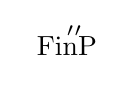
\begin{tikzpicture}[baseline=(root.base)]

    \Tree   [.\node(root){FinP};
                {Fin\\tha}
                [.TP
                    mi
                    [.T$'$
                        {T\\\tuple{tha}}
                        [.AspP
                            \tuple{mi}
                            [.Asp$'$
                                {nam[\Fsg]}
                                [.XP
                                    \tuple{mi}
                                    oileanach
                                ]
                            ]
                        ]
                    ]
                ]
            ]

\end{tikzpicture}
%\end{forest}
\z

%The \isi{movement} of the DP is also expected, on analogy with aspectually marked verbal structures, where we would, following standard practice, take the subject to be Merged below the aspectual particle, raising from its vP internal position to a higher case-related position, so that \Next would have the the analysis in \NNext, making sense of the position of the adverb :
%
%\exg. Tha Calum {an comhnaidh} ag \`ol\\
%Be.\Prs{}  Calum  always \Asp{}  drink.\Vn{} \\
%\glt \enquote*{Calum is drinking.}
%
%\ex. [\tss{TP} Tha Calum [\tss{AspP} {an comhnaidh} [\tss{AspP} ag [\tss{vP} \tuple{Calum} \`ol ]]]]

Once the subject (\emph{mi}) has raised to the specifier of TP, its trace is not counted for the calculation of labels, so the XP receives the same label as the nominal \emph{oileanach} (N).

The cleft-strategy\is{clefts} could be then taken to involve the same underlying structure,
but with \isi{movement} of the predicate NP as opposed to the subject, as follows:

\ea
%\begin{forest}
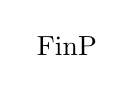
\begin{tikzpicture}[baseline=(root.base)]
    \Tree
    [.\node(root){FinP};
        {Fin\\tha}
        [.TP
            {T\\\tuple{tha}}
            [.AspP
                {nam[\Fsg{}]}
                [.XP
                    mi
                    {\tuple{oileanach}}
                ]
            ]
        ]
    ]
\end{tikzpicture}
%\end{forest}
%\begin{forest}
%[FinP
%    [Fin\\tha ]
%    [TP
%
%            [T\\{\tuple{tha}} ]
%            [AspP
%                    [ {nam[1sg]} ]
%                    [XP
%                        [ mi ]
%                        [ \tuple{oileanach} ]
%                    ]
%            ]
%    ]
%]
%\end{forest}
\z

We have seen that if the DP
subject moves, we have the p-strategy. If the DP subject stays in situ, the
predicate NP must move, on a Moro/Chomsky type analysis. That will derive
movement of the predicate NP, but leaves open the question of why Asp does not
agree in the cleft-strategy, and why the predicate A-bar extracts, rather than
moves to the specifier of TP.

On the first of these, predicates in Gaelic do not, in general, enter into
morphosyntactic \isi{agreement} with their subjects,\is{agreement!subject
agreement} so we find different inflection on attributive vs.\ predicative
adjectives, with only the former infecting for \isi{agreement}:

\ea \ili{Scottish Gaelic}
\ea \gll na caileagan m\`ora\\
the.\Pl{} girls big.\Pl{}\\
\glt \enquote*{the big girls}
\ex \gll Tha na caileagan m\`or/*m\`ora\\
be.\Prs{} the.\Pl{} girls big/*big.\Pl{}\\
\glt \enquote*{The girls are big.}
\z
\z
Since predicates do not enter into \isi{agreement}, Asp will not agree when the
predicate is extracted across it, presumably because the nominal predicate does
not, in fact, bear a full set of \isi{φ-features}.

The noun does agree with its subject in number, as we can see in examples like
the following:

\ea \ili{Scottish Gaelic}\\
\gll Tha na caileagan nan oileanaich \\
be.\Prs{} the girls in.\Poss.\Tpl{} students\\
\glt \enquote*{The girls are students.}
\z

However, this \isi{agreement} is semantic, not syntactic, as can be seen in the use
of a singular predicate nominal with plural morphosyntactic \isi{agreement} connected
to honorificity. Just as in languages like \ili{French}, the plural of the second
person is used to mark respect, but the nominal in such cases shows number
marking which is dependent on the plurality of the semantic referent (in this
case singular).

\ea \ili{Scottish Gaelic}\\
\gll Tha sibh nur oileanach \\
be.\Prs{} you in.\Poss.\Spl{} student\\
\glt \enquote*{You are a student.}
\z

I return to the importance of the semantic interpretability of number on these
nominals in adjudicating between different analytical approaches to this
construction below.

We then need an extra stipulation to force further A-bar extraction into a
cleft structure.  We do not find predicate adjectives or prepositional phrases
in subject position in Gaelic (that is, immediately following the finite
auxiliary). If that generalisation is stated across the semantic category of
predicate, rather than the syntactic category of nominal (so Gaelic would not
allow the kind of inversion of predicate to subject, discussed by
\citet{moro:97} or \citet{dendikken:06}), that would rule out the following
example (I return to this example below -- it is not as innocuous as it
appears):

\ea \ili{Scottish Gaelic}\\
\gll * Tha oileanach {ann an} Calum\\
     {} be.\Prs{} student in Calum\\
\glt \hspaceThis{*} intended: `Calum is a student.'\label{oileanach-ann}
\z
The predicate NP cannot move to the specifier of T: the predicate's
\isi{φ-features} are not sufficient to allow the kind of feature sharing that
Chomsky's system requires for specifier licensing. In such a derivation TP
would never be labelled.

We can however, allow the predicate to be directly A-bar extracted from its
base position, giving the relative clause\is{relative clauses} portion of~\eqref{relc} the structure
in~\eqref{relctree}:

\ea \ili{Scottish Gaelic} \label{relc}\\
\gll 's e oileanach a th' {ann an} Calum.\\
\Cop{} it student \Rel{} be.\Prs{} in Calum\\
\glt \enquote*{Calum is a student.}
\ex  \label{relctree}
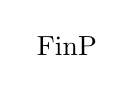
\begin{tikzpicture}[baseline=(root.base)]

    \Tree     [.\node(root){FinP};
                tha
                [.TP
                    \tuple{tha}
                    [.Asp
                        {ann an}
                        [.{\vphantom{XP}}
                            {Calum}
                            {\tuple{oileanach}}
                        ]
                    ]
                ]
            ]

\end{tikzpicture}
%\begin{forest}
%[FinP [ tha ] [TP   [ \tuple{tha} ] [Asp [ {ann an} ] [ [ {Calum} ] [ {\tuple{oileanach}} ]]]]]
%\end{forest}
\z

The full cleft\is{clefts} structure would then incorporate this relative clause\is{relative clauses} as a subpart.

This analysis seems fairly well motivated, and it captures the apparently
similar thematic relationship between the two alternative ways to express
NP-pred\-i\-ca\-tion.  However,  it turns out that there are consistent
semantic differences between the two strategies, suggesting that the underlying
configuration of the \isi{predication} is different in the two cases, as opposed to
just the surface structures. The syntactic analysis just sketched does not lead
to the expectation of such differences, and so I propose an alternative.

\section{A syntax/semantics interface analysis}

There are interesting semantic differences between the p-strategy and the
cleft-strategy, which are not connected to the information structure/focus
properties associated with \isi{clefts}. The differences are somewhat subtle, but
also familiar from NP-predicate constructions in other languages (see, for
example, \citealt{roy:06}).

The first is the oddness of~\eqref{nacatroy}, compared to~\eqref{roynacat}:

\ea \ili{Scottish Gaelic}\\
\gll ?* Tha Lilly na cat\\
    {}  be.\Prs{} Lilly in.\Poss.\Tsg.\glossF{} cat\\
\glt \hspaceThis{?*} \enquote*{Lilly is a cat}\label{nacatroy}
\ex \ili{Scottish Gaelic} \label{roynacat}\\
\gll 'S e cat a th' {ann an} Lilly\\
\Cop{} it cat \Rel{} be.\Prs{} in Lilly\\
\glt \enquote*{Lilly is a cat.}
\z
Roughly, the p-strategy is used when the assertion made by the \isi{predication} is
assumed to be non-permanent. \eqref{nacatroy} improves, for example, if we add an
adjective that restricts the predicate in a way that is sensible for a predicate
which holds only temporarily (see also \citealt{schreiner:15} for more detailed
discussion and further examples):

\ea \ili{Scottish Gaelic}\\
 \gll Tha Lilly d\`ireach na cat \`og, an drasta.\\
be.\Prs{} Lilly just in.\Poss.\Tsg.\glossF{} cat young, now\\
\glt \enquote*{Lilly is just a young cat now.}
\z
This semantic restriction is why occupations (loosely construed) tend to be the
only class of nouns used in the p-strategy in everyday discourse. NPs denoting
occupations are easily understood as temporary properties of
individuals:

\ea \ili{Scottish Gaelic}\\
\gll Tha mi nam \`oraidaiche.\\
be.\Prs{} I in.\Poss.\Fsg{} lecturer\\
\glt \enquote*{I am a lecturer}
\z
The effect is more striking when we use the two strategies to make claims about
class inclusion. It is simply impossible to use the p-strategy to express such
propositions:\footnote{\label{generic}It is possible to use the ICC
    construction, as in~\eqref{eun} (see footnote~\ref{icc}). However, the
    cleft\is{clefts} construction is much preferred in normal discourse:

\ea\label{eun}
\ili{Scottish Gaelic}\\
\gll Is eun (an) iolaire.\\
\Cop{} bird (the) eagle\\
\glt \enquote*{The eagle is a bird/An eagle is a bird.}
\z
I return to this in~\Cref{motiv2}.}

\ea \ili{Scottish Gaelic}\\
    \gll * Tha (an) iolaire na eun\\
         {} be.\Prs{} (the) eagle in.\Poss.\Tsg.\M{} bird\\
\glt \hspaceThis{*} intended: `The eagle is a bird/An eagle is a bird.'
\ex \ili{Scottish Gaelic}\\
\gll  's e eun a th' anns  an iolaire / a th' {ann an} iolaire\\
\Cop{} it bird \Rel{} be.\Prs{} in.\Def{} the eagle / \Rel{} be.\Prs{} in eagle\\
\glt \enquote*{The eagle is a bird/An eagle is a bird.}
\z
However, whereas the p-strategy is restricted in this way in its
interpretation, the cleft-strategy\is{clefts} is not. So it is perfectly well formed to
use the cleft-strategy to express class inclusion, as well as predication
involving occupations:

\ea \ili{Scottish Gaelic}\\
\gll 's e \`oraidaiche a th' annam\\
 \Cop{} it lecturer \Rel{} be.\Prs{} in.\Fsg{}\\
\glt \enquote*{I'm a lecturer.}
\z
That this semantic difference at least partially tracks the syntactic
difference between the two strategies suggests that it would be profitable to
link the syntax and semantics tightly here. In contrast to the proposal
sketched in the previous section, where the underlying structures for the two
strategies are the same, with \isi{movement} operations driving the surface
differences, I suggest instead  that there are two distinct ways of
constructing nominal \isi{predication}, correlating with the distinct interpretations
that these structures have.

Take first the p-strategy:

\ea \ili{Scottish Gaelic}\\
\gll Tha  Calum  na  oileanach.\\
Be.\Prs{}  I  in.\Poss.\Tsg.\M{}  student \\
\glt \enquote*{Calum is a student.}
\z
I propose that the p-strategy does indeed involve an aspectual particle, which
combines with a  stative category, denoted by functional structure containing
the nominal. Schematically:

\ea
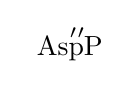
\begin{tikzpicture}[baseline=(root.base)]

    \Tree   [.\node(root){AspP};
                \edge[draw=none]; {}
                [.Asp$'$
                    {Asp\\\enquote*{in}}
                    [.StateP
                        {DP}
                        [.State$'$
                            {State}
                            {Student}
                        ]
                    ]
                ]
            ]

\end{tikzpicture}

%\begin{forest}
%[AspP
%    [Asp'     [Asp\\{`in'} ]
%            [StateP
%                [ {DP} ]
%                [State'
%                    [ {State} ]
%                         [ {Student} ]
%                ]
%            ]
%    ]
%]
%\end{forest}
\z
The  \isi{agreement} on the aspectual particle is dealt with as before. I motivated
in the last section, the idea that the P in these structures is an aspectual
particle, keyed to the aktionsart of its complement, and I will further
motivate this idea below. The noun `student' here, we shall see, cannot have
much in the way of functional structure built above it. Following
\citet{adger-ramchand:03}, I take it to denote a property.

The cleft-strategy\is{clefts}, on the other hand, involves a ``higher'' level kind of
predication:

\ea \ili{Scottish Gaelic}\\
\gll 's e oileanach a th' {ann an} Calum\\
\Cop{} it student \Rel{} be.\Prs{} in Calum\\
\glt \enquote*{Calum is a student.}
\z
I suggest for this structure that the ``subject'' is actually the NP
\emph{oileanach}, `student' and that the \isi{predication} asserts that this is in
the set (of sets) denoted by the DP \emph{Calum} (under the generalized
quantifier denotation of Calum), extending the proposals in
\citet{Adger2011b}.

%The reason that \Next is impossible, is that the NP \emph{oileanach} will be case marked in this position, and case marked NPs are interpreted as arguments, either bound by a quantifier or referential in themselves (viz. the Visibility Condition of \citep{chomsky:86a}):
%
%\exg. *Tha oileanach {ann an} Calum\\
%be.\Prs{} student in Calum\\
%intended: `Calum is a student.'
%
%For this structure to be interpretable, though, the `subject' must denote a set, not an individual.

Schematically we have:

\ea \ [\tss{CopP} \Cop{} it student]  \ [\tss{CP} [ \tuple{student} in Calum ]] \z

Following \citet{adger-ramchand:05}, the apparent expletive\is{expletives} is treated as the
predicate of the copular\is{copulas} clause, with the meaning of the relative CP being
substituted for it during the interpretation procedure.

These two structures give us a hook with which to capture the different
meanings of the p- and cleft-strategy, in that the underlying predicational
relations are differently represented. The p-strategy involves a kind of
stative \isi{predication} while the cleft-strategy\is{clefts} involves property inclusion.  I
work out the details in the next section.

%However, if this analysis is correct, it raises the question of why the USC analysis, which seems more unitary, is not viable. I will suggest that the USC analysis is impossible, because no projection of NP is ever a syntactic predicate. Take the general schema of a functional element taking a lexical category complement:
%
%\ea \  [\tss{FP} DP [\tss{F'} F XP ] ] \z
%
%My claim is that DP specifiers in the projection line of a lexical category X are only possible when F, a functional category in that projection line, has an event variable (cf. \citealt{adgerbook}). If XP here is a nominal, then an eventuality interpretation must be imposed upon it; that is, the property denoted by the root must be able to be interpreted as a temporally bounded state.

Before turning to the details and the more general implications, however, it is
necessary to show how this analysis I have just suggested is  implemented
syntactically.

\section{Motivating the interface analysis: The p-strategy}

As mentioned above, the syntax of p-strategy NP \isi{predication} constructions is
shared by the syntax of certain verbs of position. Typically, grammars of
Gaelic list nine or ten such verbs in common use, including \emph{suidh}, `sit,
\emph{seas}, `stand', \emph{duisg}, `awaken', \emph{caidil}, `sleep',
\emph{laigh}, `lie down' etc, although there are others which are rarer. Each
of these verbs actually signifies a state transition when used in the simple
past, and they can all occur with the simple aspectual particle \emph{ag},
which marks an overlap between speech and event time, with no temporal terminus
to the event time (see \citealt{adger:96,ramchand:97}).\footnote{It
is interesting that, in various dialectal varieties of English, one finds the
use of the \isi{passive} participle to mark the equivalent of the (c) examples here:
\%\emph{I was stood/sat there}.}

\ea \ili{Scottish Gaelic}
\ea \gll Shuidh mi\\
sit.\Pst{} I\\
\glt \enquote*{I sat (down).}
\ex \gll Bha mi a' suidhe\\
be.\Pst{} I \Simp{} sit.\Vn{}\\
\glt \enquote*{I sat/was sitting.}
\ex \gll Bha mi nam shuidhe\\
be.\Pst{} I in.\Poss.\Fsg{} sit.\Vn{}\\
\glt \enquote*{I was sitting/seated.}
\z
\ex \ili{Scottish Gaelic}
\ea \gll  Sheas mi\\
stand.\Pst{} I\\
\glt \enquote*{I stood (up).}
\ex \gll  Bha mi a' seasamh\\
be.\Pst{} I \Simp{} stand.\Vn{}\\
\glt \enquote*{I stood/was standing.}
\ex \gll  Bha mi nam sheasamh\\
be.\Pst{} I in.\Poss.\Fsg{} stand.\Vn{}\\
\glt \enquote*{I was standing.}\label{nam-sheasamh}
\z
\ex \ili{Scottish Gaelic}
\ea \gll  Chaidil mi\\
sleep.\Pst{} I\\
\glt \enquote*{I fell asleep.}
\ex \gll Bha mi a' cadal\\
be.\Pst{} I \Simp{} sleep.\Vn{}\\
\glt \enquote*{I slept/was falling asleep.}
\ex \gll Bha mi nam chadal\\
be.\Pst{} I in.\Poss.\Fsg{} sleep.\Vn{}\\
\glt \enquote*{I was sleeping/asleep.}
\z
\z
Simple stative verbs, such as \emph{ciallaich}, `mean', \emph{faic}, `see' and
\emph{cr\`eid}, `believe', are perfectly well formed with the simple aspectual
particle, but not with the various forms of \emph{ann an} in its aspectual
incarnation:

\ea \ili{Scottish Gaelic}
\ea[]{\gll D\`e tha sin a' ciallachadh\\
what be.\Prs{} that \Simp{} mean.\Vn{}\\
\glt \enquote*{What does that mean?}}
\ex[*]{\gll D\`e tha sin na ciallachadh\\
what be.\Prs{} that in.\Poss.\Tsg{} mean.\Vn{}\\
\glt intended: `What does that mean?'}
\z\z
The crucial difference between simple statives and the stative verbs of
position is that the latter involve a change of state followed by a temporary
steady-state result of that change while the former do not specify any
transitions at all. That is, the verbs of position are interval statives
(\citealt[184]{Dowty:1979}) and the contribution of \emph{ann an} is to signal
that the \isi{predication} is included in the interval. If we think of this using a
locational metaphor, the state is represented as characterizing a temporal
location for the subject.

If this characterization is correct, then we expect to see the \emph{ann an}
structure used when the action that leads to the steady-state is in fact
non-canonical for such actions (for example, one can be standing even though
the event that leads to this state is not an event of standing up). This is
correct:

\ea \ili{Scottish Gaelic}\\
 \gll Dh'\`eirich e na shuidhe\\
rise.\Pst{} he in.\Poss.\Tsg.\M{} sit.\Vn{}\\
\glt \enquote*{He sat up (literally, he rose in his sitting).}
\ex \ili{Scottish Gaelic}\\
\gll  Leum mi nam sheasamh\\
jump.\Pst{} I in.\Poss.\Fsg{} stand.\Vn{}\\
\glt \enquote*{I jumped to a standing position (literally, I jumped in my standing).}\label{leum}
\z
This kind of data strongly suggests a kind of event decomposition, as argued
for by \citet{ramchand08}: the state in which the subject is asserted to be is
separated from the (sub-)event that initiates it in examples like these.

What of the kind of NP \isi{predication} that we find in the p-strategy. Here too,
the subject is characterized as being in a state which has a transitory nature.
We can see this by using the standard temporal modifier test:

\ea \ili{Scottish Gaelic}\\
 \gll  Bha Iain na shuidhe fad uair a th\`ide\\
be.\Pst{} Iain in.\Poss.\Tsg.\M{} sit.\Vn{} length hour of time\\
\glt \enquote*{Iain was sitting for an hour.}
\ex \ili{Scottish Gaelic}\\
\gll  Bha Iain na oileanach fad d\`a bhliadhna\\
be.\Pst{} Iain in.\Poss.\Tsg.\M{} sit.\Vn{} length two year\\
\glt \enquote*{Iain was a student for two years.}
\z
If this semantic characterization is correct, it will explain the oddness
of~\eqref{nacat2} as a result of the knowledge that one is not usually a cat for a
temporary period, that is, it is equivalent to the oddness of~\eqref{englnacat} in
English:

\ea \ili{Scottish Gaelic}\\
    \gll ?* Tha Lilly na cat\\
         {} be.\Prs{} Lilly in.\Poss.\Tsg.\glossF{} cat\\
    \glt \hspaceThis{?*} \enquote*{Lilly is a cat}\label{nacat2}
\ex[?*]{Lilly is a cat for an hour.}\label{englnacat}
\z
From this perspective, \eqref{nacat2} is actually perfectly grammatical, but it is
inconsistent with what we know about what it means to be a cat, hence the
acceptability judgment given. In fact, one of my consultants said that this
sentence was fine if Lilly was a shape-changer, to express which she used the
cleft-strategy!

\ea \ili{Scottish Gaelic}\\
\gll  nam b' e shape-changer a bh' innte\\
if \Cop.\Cond{} it shape-changer \Rel{} be.\Pst{} in.\Tsg.\glossF{}\\
\glt \enquote*{if she was a shape-changer.}
\z
This approach will also explain why verbal states such as \emph{ciallaich},
`mean' (which lack such transitions) are impossible in p-strategy type
structures, since \emph{ann an} requires a state which has the appropriate
interval property.

%I will implement the idea of interval stativity through a State head in the syntax. This combines with a piece of syntactic structure that can be interoreted as an interval state. Certain verbs are very natural interval states, and hence appear in this construction. Most nominals are not construed as interval states, but can be coerced into such an interpretation (as in the `cat' example immediately above), but some easily accept such an interpretation.
%
%The State head has a semantics which predicates the nominal property of an stative event:
%
%\ex. \sem{State} = $\lambda$P$\lambda$s.holds(P, s)
%
%This is almost identical to the meaning given by \citep{adger-ramchand:03} to the copular\is{copulas} Pred head that appears in the archaic copular\is{copulas} constructions. The difference is that that head specifies a {\bf holds} relation between a nominal property and an individual variable, while State specifies the relation between a nominal property and a state.

%I turn now to the hypothesized inherent reflexiveness of this kind of \isi{predication}.

%The verbs of position have a further characteristic beyond their interval nature: the subject of the initiating sub-event which leads to the state of, for example, sitting, is necessarily the same as the subject of the state of sitting, at least in Gaelic. Unlike in English, these verbs do not causativize:
%
%\exg. *Sheas mi suas e\\
%Stood I up it\\
%intended: `I stood it up'
%
%\exg. *Laigh mi s\`ios i\\
%Lay I down her\\
%intended: `I lay her down'
%
%Moreover, even when the initiating action is separately identified, it must have the same subject as the state:
%
%\exg. *Dh'\`eirich e nam shuidhe\\
%rise.\Pst{} he in.\Poss.\Fsg{} sit.\Vn{}\\
%intended: `He sat me up (literally, he rose in my sitting).'
%
%\exg. *Leum mi na seasamh\\
%jump.\Pst{} he in.\Poss.\Tsg.\glossF{} stand.\Vn{}\\
%intended: `I jumped her up to a standing position (literally, I jumped in her standing).'\label{leum2}

%It appears, then, that these verbs of position involve an inherent control relation between the two sub-events, reminiscent of manner of motion verbs involving bodyparts:
%
%\ex. \a. I shrugged my/*his shoulders
%\b. She tossed her/*my hair
%
%In \Last, the bodypart undergoing \isi{movement} is under the control of the entity of which it is a part. This is not true of all verbs of \isi{movement}:
%
%\ex. \a. I moved my/his shoulders.
%\b. She turned her/my head.
%
%I take this kind of effect to motivate the presence of a reflexive pronominal
%in the state \isi{predication}, although no doubt more needs to be said about
%the ``control'' relation. To implement this, I will assume that the reflexive pronominal is obligatorily Merged as the specifier of a State head, which is the complement of an aspectual projection headed by \emph{ann an}. This aspectual projection is responsible for the entailment that the state is the result of some transition (that is, it forces a target state reading \`a la \citep{parsons:90}):\footnote{An alternative to this representation would be to generate \emph{ann an} lower, as the head of State, then raise it to Asp. This would allow the statement of the reflexive constraint on the external argument to be more directly specified as a property of just this functional head, rather than as a selectional relation between \emph{ann an} and different kinds of state (interval vs non-interval). The lexical content of the state could then be Merged as the complement of State.}

I analyse the syntax of these stative verbs of position by assuming the existence of a St
functional category. St creates a bounded interval over which the property
denoted by the root holds. Bounded temporal intervals are a kind of eventuality
or situation. So I assume, like v, this category has an event variable, and
introduces a specifier subject. I'll assume this is done via
event-identification (\citealt{kratzer96}), but an implementation in the
theory of \citet{ramchand08} is equally doable.

The relationship between the interval state given by the St head and the
temporal structure of the remainder of the sentence is negotiated by Asp.

\ea
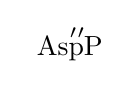
\begin{tikzpicture}[baseline=(root.base)]

    \Tree     [.\node(root){AspP};
                {Subj}
                [.Asp$'$
                    {ann an}
                    [.StP
                        \tuple{Subj}
                        [.St$'$
                            {St}
                            {root}
                        ]
                    ]
                ]
            ]

\end{tikzpicture}
%\begin{forest}
%[AspP [ {Subj} ] [Asp' [ {ann an} ] [StP [ \tuple{Subj} ] [St' [ {St} ]  [
%{root} ]]]]]
%\end{forest}
\z
This structure can be embedded under an initiating eventuality. In the case
where that eventuality is a verb like `jump' as in~\eqref{leum} above, we
have~\Cref{tree1}, where AspP is the complement of the aspectual structure of
\emph{leum}, `jump' (for concreteness I assume the subject raises to its
(nominative) case marking position, the specifier of TP,
with the finite verb raised to Fin \citealt{adger:07}).

\begin{figure}
\caption{Structure of example \eqref{leum}.\label{tree1}}
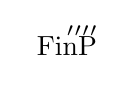
\begin{tikzpicture}[baseline=(root.base), scale=.9]
    \Tree     [.\node(root){FinP};
                {leum}
                [.TP
                    {mi}
                    [.T$'$
                        \tuple{leum}
                        [.vP
                            \tuple{mi}
                            [.v$'$
                                \tuple{leum}
                                [.VP
                                    \tuple{leum}
                                    [.AspP
                                        \tuple{mi}
                                        [.Asp$'$
                                            {ann an[\Fsg]}
                                            [.StP
                                                \tuple{mi}
                                                [.St$'$
                                                    {St}
                                                    {seasamh}
                                                ]
                                            ]
                                        ]
                                    ]
                                ]
                            ]
                        ]
                    ]
                ]
            ]
\end{tikzpicture}
\end{figure}
%\begin{forest}
%[FinP [ {leum} ] [TP [ {mi} ] [T' [ \tuple{leum} ]  [vP [ \tuple{mi} ] [v' [ \tuple{leum} ] [VP [ \tuple{leum} ]  [AspP [ \tuple{mi}]  [Asp' [ {ann an[1sg]} ] [StP [ \tuple{mi} ] [St' [ {St} ] [ {seasamh} ]]]]]]]]]]]
%\end{forest}

Agreement appears on Asp as a reflex of the \isi{movement} operation affecting the
subject, as in~\Cref{tree1}.

In the situation where the verbal root is compatible with a process, Asp takes
the verbal root directly (or a VP built from it), and introduces the subject via the aspectual head
\emph{ag/a'}, which signifies that the interpretation involves a process, as we
saw above; see~\Cref{ag-tree}:

\ea \ili{Scottish Gaelic}
\ea\gll Bha mi a' suidhe\\
be.\Pst{} I \Simp{} sit.\Vn{}\\
\glt \enquote*{I sat/was sitting.}\label{adger:56a}
\ex \gll Bha mi nam shuidhe\\
be.\Pst{} I in.\Poss.\Fsg{} sit.\Vn{}\\
\glt \enquote*{I was sitting/seated.}
\z
\z

\begin{figure}
\caption{Structure of example \eqref{adger:56a}.\label{ag-tree}}
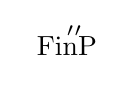
\begin{tikzpicture}[baseline=(root.base)]

    \Tree     [.\node(root){FinP};
                bha
                [.TP
                    mi
                    [.T$'$
                        \tuple{bha}
                        [.AspP
                            \tuple{mi}
                            [.Asp$'$
                                a'
                                suidhe
                            ]
                        ]
                    ]
                ]
            ]

\end{tikzpicture}
%\begin{forest}
%[FinP
%    bha
%    [TP    mi
%        [T'
%            \tuple{bha}
%            [AspP
%                \tuple{mi}
%                [Asp'
%                    a'
%                    suidhe
%                ]
%            ]
%        ]
%    ]
%]
%\end{forest}
\end{figure}

The general framework here follows Ramchand's in assuming that verbal\linebreak meanings,
including the aspectual meanings and introduction of arguments are distributed
across various syntactic elements (see also \citealt{Borer2005}).
%ANDRAS: check in refs. Borer, Hagit 2005 The Normal Course of Events Oxford University Press, Oxford.

Following this general framework, simple state verbs, like `mean', `see', `believe', etc., also generate their
subject in the specifier of AspP, rather than as a subject of St, much like
process verbs, so~\eqref{adger:57} has the structure in~\Cref{ag-tree2}.\pagebreak

\ea \ili{Scottish Gaelic}\label{adger:57}\\
\gll Tha mi a' faicinn a' chait\\
be.\Prs{} I \Simp{} see.\Vn{} the.\Gen{} cat.\Gen{}\\
\glt \enquote*{I see the cat.}
\z

\begin{figure}
    \caption{Structure of example~\eqref{adger:57}.\label{ag-tree2}}
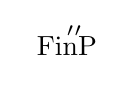
\begin{tikzpicture}[baseline=(root.base)]

    \Tree 	[.\node(root){FinP};
                tha
                [.TP
                    mi
                    [.T$'$
                        \tuple{tha}
                        [.AspP
                            \tuple{mi}
                            [.Asp$'$
                                a'
                                [.VP
                                    faicinn
                                    [.DP
                                        a' chait
                                    ]
                                ]
                            ]
                        ]
                    ]
                ]
            ]

\end{tikzpicture}
%\begin{forest}
%[FinP
%    tha
%    [TP    mi
%        [T'
%            \tuple{tha}
%            [AspP
%                \tuple{mi}
%                [Asp'
%                    a'
%                    [VP
%                        faicinn
%                        [DP a' chait ]
%                        ]
%                ]
%            ]
%        ]
%    ]
%]
%\end{forest}
\end{figure}

For the verbs of position in their stative incarnation that we are
concentrating on here, then, AspP is then Merged with TP,
giving \Cref{suidhetree} as a representation for~\eqref{suidhe}:

\ea \ili{Scottish Gaelic} \label{suidhe}\\
 \gll  Bha mi nam shuidhe\\
be.\Pst{} I in.\Poss.\Fsg{} sit.\Vn{}\\
\glt \enquote*{I was sitting/seated.}
\z

\begin{figure}
\caption{Structure of example~\eqref{suidhe}.\label{suidhetree}}
\begin{tikzpicture}[baseline=(root.base)]

    \Tree 	[.\node(rote){FinP};
                bha
                [.TP
                    mi
                    [.T$'$
                        \tuple{bha}
                        [.AspP
                            \tuple{mi}
                            [.Asp$'$
                                {ann an}
                                [.StP
                                    \tuple{mi}
                                    [.St$'$
                                        St shuidhe
                                    ]
                                ]
                            ]
                        ]
                    ]
                ]
            ]

\end{tikzpicture}
%\begin{forest}
%[FinP [ bha ] [TP [ mi ] [T' [ \tuple{bha} ] [AspP [ \tuple{mi} ] [Asp' [ {ann
%an} ] [StP [ \tuple{mi} ] [St' [ St ] [ shuidhe ]]]]]]]]
%\end{forest}
\end{figure}

With this syntax for interval statives in hand, the reason why Gaelic uses this\largerpage
structure, and why Gaelic nominal \isi{predication} has restricted interpretation can
be understood to derive from a basic difference in how nouns and verbs work.
The theory developed in \citet{adgerbook} takes nouns to be simple sortal
predicates of individuals, and verbs to be predicates of eventualities. Indeed,
in that theory, the roots are directly contained in a category N or V whose
semantics is to introduce either an individual or an event variable.

{\sloppy
However, events have a semantic combinatory capacity to license arguments which
are interpreted as participants of the event. This can be done either via some
rule of event-identification (\citealt{kratzer96}), or via a semantics which
takes the extended projection of V to describe event structure
directly \parencite{ramchand08}. Whatever the implementation, we can strengthen
these proposals to the following:}

\ea For an XP to act as a syntactic predicate, licensing an argument, it must
have a semantically open eventuality variable. \z

If we put this proposal together with the idea that nouns are simple sortal
predicates of individuals, the upshot is that apparent arguments of nouns have
to be introduced as modifiers, while those of verbs can be introduced as
specifiers. \textcite{adgerbook} uses this theory to explain why apparent
arguments to nominals behave so differently to arguments to verbs in terms of
their licensing, optionality and syntactic position. However, there is a
further consequence not explored in \citet{adgerbook}: nominal predication
cannot involve simply projecting a subject to a noun, as nouns cannot license
arguments:

\ea
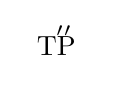
\begin{tikzpicture}[baseline=(root.base)]

    \Tree 	[.\node(root){TP};
                Calum
                [.T$'$
                    is
                    [.NP
                        \tuple{Calum}
                        [.N$'$ {N\\student}
                        ]
                    ]
                ]
            ]

\end{tikzpicture}
%\begin{forest}
% [TP [ Calum ] [T' [ is ] [NP [ \tuple{Calum} ] [N' [N\\student ]]]]]
%\end{forest}
\z

Since there is no event variable here, Calum cannot be the syntactic subject of a nominal predicate. This is the reason why simple nominal \isi{predication} is impossible in Gaelic:

\ea \ili{Scottish Gaelic}\label{adger:61}\\
    \gll * Tha  Calum  oileanach.\\
         {} Be.\Prs{}  Calum student \\
    \glt \hspaceThis{*} \enquote*{Calum is a student.}
\z

The solution that Gaelic adopts is to allow St to combine with the root nominal
first, as shown in \Cref{fig:adger:GaelicSt} and \REF{adger:ex:62}.

\begin{figure}
\caption{Structure of example~\eqref{adger:ex:62}.\label{fig:adger:GaelicSt}}
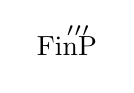
\begin{tikzpicture}[baseline=(root.base)]

    \Tree 	[.\node(root){FinP};
                tha
                [.TP
                    {Calum}
                    [.T$'$
                        \tuple{tha}
                        [.AspP
                            \tuple{Calum}
                            [.Asp$'$
                                {Asp\\{ann an}}
                                [.StP
                                    \tuple{Calum}
                                    [.St$'$
                                        St
                                        oileanach
                                    ]
                                ]
                            ]
                        ]
                    ]
                ]
            ]

\end{tikzpicture}
%\begin{forest}
%[FinP [ tha]  [TP [ Calum ] [T' [ \tuple{tha} ] [AspP [ \tuple{Calum} ] [Asp' [Asp\\{ann an} ] [StP [ \tuple{Calum} ] [St' [ St ] [ oileanach ]]]]]]]]
%\end{forest}
\end{figure}

\ea \ili{Scottish Gaelic}\label{adger:ex:62}\\
 \gll  Tha Calum na oileanach\\
be.\Prs{} Calum in.\Poss.\Tsg.\M{} student\\
\glt \enquote*{Calum is a student.}
\z
Here the root \emph{oileanach}, `student', is a property. Usually it will
combine with a categorizer like n (or just N in \citeauthor{adgerbook}
\citeyear{adgerbook}'s theory) which
associates it with an individual level variable:\largerpage

\ea \sem{N} = $\lambda$P$\lambda$x.holds(P, x) \z
However, St combines with this property, associating it with a variable which
ranges over temporally bounded states (cf. Carlsonian stages,
\citealt{carlson:77}). I will represent such variables as s:

\ea \sem{St} = $\lambda$P$\lambda$s.holds(P, s) \z
Temporally bounded intervals, even if they are temporally bounded intervals of
individuals,  are a sort of eventuality. This will allow a subject to be Merged to the (now non-nominal)
predicate. The linkage between the nominal and the verbal here is, then,
because the functional category St generates temporally bounded states, which
are a kind of eventuality, even if the state is actually a stage of an
individual.\largerpage

This theory makes a prediction that modifiers which require an individual
variable should be impossible in such structures. For example, relative
clauses, which require a modification relation to be set up over individual
variables, will be ruled out, as these structures never contain an individual
level variable. This turns out to be correct:\footnote{Many thanks to Jason
Ostrove for testing a number of these examples for me while on fieldwork in the
Hebrides.}

%'Se comhairle a tha na phiuthair a gheibh a' vote agam. (or "a thaghainn")
%'S e comhairle a tha na phiuthair. Gheibh i a' vote agam.
\ea \ili{Scottish Gaelic}\\
    * \parbox[t]{\linewidth - \widthof{* }}{\gll  Tha a phiuthair na comhairle a gheibh a' vote agam. \\
           be.\Prs{} her sister in.\Poss.\Tsg.\glossF{} councillor that get.\Fut{} the vote at.\Fsg{}\\
    \glt \enquote*{His sister is a councillor who I will vote for.}}
\z
Here, \emph{ann an} combines with StP, which denotes a temporally bounded
period of an individual (a stage), not an individual. A relative clause\is{relative clauses}
combines with an individual (via predicate modification), and hence is
impossible here.

A restricted range of modifiers that can work at the stage level, such as
\emph{\`ur}, `new', are correctly predicted to be acceptable:

\ea \ili{Scottish Gaelic}\\
\gll Tha Calum na oileanach \`ur\\
be.\Prs{} Calum in.\Poss.\Tsg.\M{} student new\\
\glt \enquote*{Calum is a new student}
\z
The adjective \emph{\`ur}, `new', modifies a temporal aspect of being a
student, and hence is acceptable.

This approach also predicts the absence of quantifiers and
numerals in the Gaelic structures.  Even though \isi{numerals} and weak quantifiers are usually\linebreak
thought of as maintaining the predicative type of an NP, they are impossible in the
p-strategy.

\ea \ili{Scottish Gaelic}
\ea[*]{\gll Bha iad nan c\`oig oileanaich\\
be.\Pst{} they in.\Poss.\Tpl{} five students\\
\glt \enquote*{They were five students.}}
\ex[*]{\gll Bha iad nam m\`oran oileanaich\\
be.\Pst{} they in.\Poss.\Tpl{} many students\\
\glt \enquote*{They were many students.}}
\z \z
The effect follows straightforwardly on the account given here: stages are things that can't be counted (numerals and quantifiers,
again, require individual variables).

The fact that these \isi{numerals} are possible in the cleft-strategy provides a further argument against the unified analysis of the two strategies that I sketched in section~\eqref{pred-inv}:

\ea \ili{Scottish Gaelic}
\ea \gll   's e c\`oig oileanaich a bh' annta\\
\Cop{} it five students \Rel{} be.\Prs{} in.\Tpl{}\\
\glt \enquote*{They were five students.}
\ex \gll  's e m\`oran oileanaich a bh' annta\\
\Cop{} it many students \Rel{} be.\Prs{} in.\Tpl{}\\
\glt \enquote*{They were many students.}
\z \z

\textcite{schreiner:15} presents an analysis of the p-strategy that covers
some of the same empirical ground as that presented here. She develops the
proposals of \textcite{roy:06}, arguing that nominals, in general, have an
event variable, and that different kinds of functional structure generated
above Ns give rise to the interval stative property. In Gaelic predicative
structures, the nominal has to denote what Roy calls a dense predicate
(essentially, dense predicates are temporally homogenous; they are analogous to
mass predicates, which are homogeneous in mereological structure).

Schreiner's syntactic analysis takes the constituent headed by \emph{ann an} in
the p-strategy to be a true PP, with a full DP as its complement. This DP
obligatorily has a possessor\is{possessors} inside it, which is responsible for the \isi{agreement}
on \emph{ann an}. However, this is inconsistent with the restricted
set of modifiers that these nominal predicates allow. While the absence of
numerals is expected, if nominal roots in these structures have to be
homogeneous, the absence of relative clauses is surprising (relatives are well
formed with mass nominals, of course).

To a certain extent, Schreiner's  analysis and mine are compatible in terms of
the interpretations available for the nominal predicate, as both rely on a
specialised functional structure generated above the nominal root. However,
because, for Schreiner, Ns have an event variable, her analysis  doesn't
provide a straightforward explanation for the impossibility of simple NP
predication as in~\eqref{bare}, which I take to be a desideratum:

\ea \ili{Scottish Gaelic}\\
    \gll * Tha  Calum  oileanach.\\
         {} Be.\Prs{}  Calum student \\
\glt  \hspaceThis{*} \enquote*{Calum is a student.}\label{bare}
\z

Schreiner suggests that this may have something to do with transnumerality in
the language, and suggests that nouns in Gaelic are number neutral (unspecified
for number). However, most nominals in Gaelic, and certainly all the ones in
the examples discussed here, work morphologically and semantically as simple
count or mass nominals. Strikingly, when the subject is plural, the predicate
nominal has to be plural too:

\ea \ili{Scottish Gaelic} \label{teenagers}
\ea \gll  Tha sinn nar deugairean\\
be.\Prs{} we in.\Poss.\Fpl{} teenager.\Pl{}\\
\glt \enquote*{We are teenagers.}
\ex \gll Tha i na deugaire\\
be.\Prs{} she in.\Poss.\Tsg.\glossF{} teenager \\
\glt \enquote*{She is a teenager.}
\z \z
We can make sense of this if the root, in fact, bears a plural property (e.g.
it will apply to some non-atomic point in a lattice, as in \citealt{Link:1983}) vs.
a singular property. This means that when the predicate applies to the s
variable via St, it is a predicate of stages of multiple individuals. I don't
see how these facts about number marking on the predicate nominal can be made
compatible with a proposal that nouns are number neutral. These facts are even
more striking given the impossibility of number agreement\is{agreement!number agreement} (or any
φ-agreement) on predicate adjectives:

\ea \ili{Scottish Gaelic} \label{number}
    \ea[]{\gll  na balaich m\`ora\\
    the.\M.\Pl{} boy.\Pl{} big-\Pl{}\\
    \glt \enquote*{The big boys.}}
    \ex[]{\gll Tha na balaich m\`or\\
    be.\Prs{} the.\M.\Pl{} boy.\Pl{}  big\\
`The boys are big.'}
    \ex[*]{\gll Tha na balaich m\`ora\\
    be.\Prs{} the.\M.\Pl{} boy.\Pl{}  big-\Pl{}\\
\glt intended: `The boys are big.'}
    \z
\z
Adjectives agree in number in attributive position, but not in
predicate position. Predicate position, then, is not accessible to \isi{agreement}
(which conforms with the generalization that verbs do not agree with their
subjects in Gaelic). But then that suggests that number in examples
like~\eqref{teenagers} is semantically interpreted, and that nouns are not number
neutral. An account of the impossibility of simple nominal \isi{predication} in Gaelic resting on the idea that nouns are number neutral is untenable.

 %
%\exg. Bha mi nam sheasamh aig an doras\\
%be.\Pst{} I in.\Poss.\Fsg{} stand.\Vn{} at the door\\
%`I was standing at the door.' \label{standingatthedoor}
%
%However, it's not clear to me how to implement this straightforwardly for nominal predicates, which allow at least some adjectives:
%
%\exg. Tha Calum na oileanach \`ur \\
%be.\Prs{} Calum in.\Poss.\Tsg.\M{} student new\\
%`Calum is a new student.'
%
%For this reason, I take the NP to be the complement of the stative head, creating a sort of light verb construction, where the light verb is null (this is, in a sense, a syntacticization of Chierchia's \citeyear[204]{chierchia:95generic} suggestion that nominals come in two types, one of which involves a state variable):

%%\ex.
%%\begin{forest}
%%[.FinP tha [.TP Calum[φ:3s] [.T' \tuple{tha} [.AspP  \tuple{Calum[φ:3s]} [.Asp' {ann an} [.StP pro[Refl:3s] [.St' St \qroof{oileanach \`ur}.NP  ] ] ] ] ] ] ]
%%
%%This predicts that locatives in the verbs of position and those in the superficially nominal structures should be different beasts, and this appears to be correct:
%%
%%\exg. Bha Calum na oileanach \`ur aig an doras\\
%%be.\Pst{} Calum in.\Poss.\Tsg.\M{} student new at the door\\
%%`Calum is a new student at the door.'
%%
%%The locative PP in \Last does not locate the state of being a new student, unlike the locative in~\eqref{standingatthedoor}, which does locate the state of standing.
%
\section{Motivating the interface analysis: The cleft-strategy}\label{motiv2}\largerpage[-1]

I turn now to the cleft-strategy\is{clefts}. The claim here is that the apparent predicate
is a subject, but it is the subject of a higher level \isi{predication}. That is, it
is similar to the copular\is{copulas} \isi{predication} mentioned in footnote~\ref{generic}:

\ea \ili{Scottish Gaelic} \label{sgarbh}\\
\gll   Is eun sgarbh\\
\Cop{} bird cormorant\\
\glt \enquote*{A cormorant is a bird} (Generic)
\z
In~\eqref{sgarbh} the subject NP \emph{sgarbh}, `cormorant' is asserted to be in
the set (of sets) denoted by the predicate \emph{eun}, `bird'.

\citet{adger-ramchand:03} argue that this kind of structure involves a
predicational head which raises to a higher position, pied-piping its
complement, and creating a predicate inversion structure:

\ea \label{copularinversion}
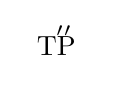
\begin{tikzpicture}[baseline=(root.base)]

    \Tree 	[.\node(root){TP};
                [.Pred$'$
                    is
                    eun
                ]
                [.PredP
                    sgarbh
                    {Pred$'$\\\tuple{is eun}}
                ]
            ]

\end{tikzpicture}
%\begin{forest}
%[TP [Pred' [ is ] [ eun ] ] [PredP [ sgarbh ] [Pred'\\{\tuple{is eun}} ]]]
%\end{forest}
\z

The predicational head is \emph{is}. Adger and Ramchand give \emph{is} a semantics which allows it to combine with a nominal, and assert that the property the nominal denotes holds of a subject as follows.\largerpage[-1]

\ea $\lambda$P$\lambda$x.holds(P, x) \z

The motivation for this semantics is that \emph{is} cannot occur in tensed sentences. It has only two forms: \emph{is}, which marks that the proposition currently holds, and \emph{bu}, which marks that it doesn't currently hold. It may have held in the past, be going to hold in the future, or be a possibility. This copular\is{copulas} element then seems to mark a distinction which
is close to a notion of ``current actuality'', perhaps to be related to evidentiality.

Importantly, for the claims I am making here, the copular\is{copulas} structure in Gaelic
does not involve \isi{predication} in the normal sense: the ``subject'' is not
a participant in a situation and is not a thematic argument of the apparent
predicate. Rather the copula\is{copulas} here denotes a pure inclusion
relation: the set of cormorants is in the set of birds. The label Pred here,
then, is somewhat misleading, and I'll replace it with simply Cop.

Adger and Ramchand extend their idea to apparent equatives in Gaelic, which have a surface
form reminiscent of \isi{clefts}:

\ea \ili{Scottish Gaelic}\\
\gll  's e  Calum an oileanach\\
Cop.\Prs{} it Calum the student\\
\glt \enquote*{Calum is the student.}
\z
We argued that in these constructions the pronominal
element \emph{e} acts as the complement to the copula\is{copulas}. This pronoun is then
anaphoric to a right adjoined definite DP:\is{adjunction}

\ea
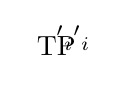
\begin{tikzpicture}[baseline=(root.base)]

    \Tree 	[.\node(root){TP};
                [.TP
                    {Cop$'$\\is e$_{i}$}
                    [.CopP
                        Calum
                        {Cop$'$\\\tuple{is e}}
                    ]
                ]
                {DP$_{i}$\\an oileanach}
                ]
            ]

\end{tikzpicture}
%\begin{forest}
%[TP [TP [Cop'\\ is e$_{i}$ ] [CopP [ Calum ] [Cop'\\{\tuple{is e}} ]]] [DP$_{i}$\\{an oileanach} ]]
%\end{forest}
\z
Equatives, then, do not exist and equative meanings are constructed via
a copular\is{copulas} structure plus an anaphoric dependency.

My suggestion here is simply to extend this idea to true \isi{clefts}, and
specifically to \isi{clefts} that involve apparent NP predicates. The
copula\is{copulas} signals inclusion of one class in another
in~\eqref{sgarbh}, and it performs an identical function
in the cleft-strategy\is{clefts} for nominal \isi{predication}.

There are two analytical premisses that underlie this claim: the first is an analysis of the syntax and semantics of the relative clause\is{relative clauses} part of the cleft-strategy; the second is an analysis of what motivates the obligatory nature of
the clefting process.

The first premiss is fairly straightforward to motivate: the preposition
\emph{ann an} in the relative clause\is{relative clauses} portion of the cleft-strategy behaves, as
we have seen, like a normal preposition, so we can assume it is syntactically a
true preposition with a DP complement. That is, we have the following syntactic
structure:

\ea {}[\tss{PredP} NP [\tss{Pred'} Pred [\tss{PP} in DP ]]] \z

The associated semantics to be justified is that this PP functions as a
predicate for a property-denoting subject NP. That is, the DP here is a
generalized quantifier, denoting a set of properties and the whole structure is
interpreted as asserting that the set of properties denoted by the NP is
included in this. This is similar to the copula\is{copulas}, but involves the situational
variable usually connected to PP \isi{predication}.

However, this seems inconsistent with an observation discussed
in~\Cref{pred-inv}. There I showed that structures of the following sort
cannot be used to make a nominal predication:

\ea \ili{Scottish Gaelic}\\
    \gll * Tha oileanach {ann an} Calum\\
         {} be.\Prs{} student in Calum\\
\glt    \hspaceThis{*} intended: `Calum is a student.'\label{inverse}
\z
This claim, although true, is not the whole story. In fact this kind
of structure can be used to say that Calum has student qualities, although he
is not a student. For example, if Calum is a one-year old child, but likes
playing with books, then \eqref{inverse} is an appropriate comment. So the * judgment in \eqref{inverse} refers not to a structural impossibility, but to an impossible reading for that structure. It is in fact well formed with the reading that Calum has student qualities.

Similarly, one can say:

\ea \ili{Scottish Gaelic} \label{bighead}\\
\gll  Tha ceann m\`or {ann an} Calum\\
be.\Prs{} head big in Calum\\
\glt  `Calum is big-headed.'
\z
\eqref{bighead} cannot mean that Calum literally has a big head, but it can mean
that he has the qualities associated with big-headedness. In fact, this
structure can be used to state that the complement of the P has the inherent
quality denoted by the NP in general. Let us roughly symbolize this
as~\eqref{qual}, where the function Qual returns a set of properties associated
with the property denoted by the NP.

\ea \label{qual} Qual(NP) is a set of properties such that each property is characteristic of the individuals denoted by NP
\z
This kind of \isi{predication} is equivalent to that seen in English constructions
like \eqref{engl}:

\ea \label{engl} I see an excellent king in Jason. \z
Here Jason is not necessarily a king, and certainly not an excellent one, but
he has the qualities necessary to be one.

The interpretations of sentences like \eqref{bighead} motivate the idea that the relative clause\is{relative clauses} part of the cleft-strategy has a syntax involving an NP subject with a PP predicate and a semantics where the NP subject denotes a set of properties asserted to be included in the properties denoted by the complement of the preposition \emph{ann an}.

The second part of the analysis that still needs to be explained is why the relativization is obligatory. Why doesn't Gaelic just allow \eqref{inverse} with the meaning `Calum is a student'?

The answer to this is that the peculiar quality reading of these NP subjects is lost whenever the quality denoting NP is extracted.

Both of the following examples have only literal readings:

\ea \ili{Scottish Gaelic}\\
\gll * D\`e an oileanach a th' {ann an} Calum\\
     {} What the student \Rel{} be.\Prs{} in Calum\\
\glt \hspaceThis{*} intended: `What kind of student is Calum?'
\ex  \ili{Scottish Gaelic}\\
\gll * 'S e ceann m\`or a th' {ann an} Calum\\
     {} \Cop{} it big head that be.\Prs{} in Calum\\
\glt \hspaceThis{*} intended: `It's big-headed that Calum is'
\z
The reason for this is not entirely obvious, but the generalization is clear,
and constitutes the second step of the argument for justifying the analysis
presented here:

\ea \label{noqual} Qual cannot apply to an A-bar bound element.\z

This seems to be true in English as well.  The relevant reading is only preserved under extraction when the noun `kind' is used:

\ea
    \ea[]{What kind of a king do you see in Jason?}
    \ex[*]{What king do you see in Jason?}
    \z
\z

Similarly for Gaelic:

%\exg. D\`e an se\`orsa oileanach a th' {ann an} Calum\\
%What the sort student \Rel{} be.\Prs{} in Calum\\
%`What kind of a student is Calum.'

\ea \ili{Scottish Gaelic}\\
    \gll D\`e an se\`orsa oileanach a th' {ann an} Calum\\
        What the sort student \Rel{} be.\Prs{} in Calum\\
    \glt \enquote*{What kind of a student is Calum.}
\ex \ili{Scottish Gaelic}\\
    \gll * D\`e an oileanach a th' {ann an} Calum\\
         {} What the student \Rel{} be.\Prs{} in Calum\\
    \glt \hspaceThis{*} intended: `What kind of student is Calum?'
\z

I'll follow \citet{adger-ramchand:05} and \citet{Adger2011} here and
take the view that wh-movement, relativization\is{relative clauses} and clefting in Gaelic all
involve an A-bar bound bare resumptive pronoun,\is{resumptive pronouns} although nothing about the
story presented here changes if we have, instead, a trace of A-bar \isi{movement}.

With these two analytical premisses in place, we can
now take~\eqref{sem1} to be the base structure to which the cleft\is{clefts} applies:

\ea \label{sem1} \gll  Tha pro {ann an} Calum = $\wp \in \lambda$P.P(Calum)\\
be.\Prs{} pro in Calum\\
\z

Here the pronominal is an NP, and its interpretation is as a variable ($\wp$) ranging over properties. The preposition \emph{ann an} asserts that whatever property is assigned to pro will be included in the set of properties denoted by Calum. The structure here is the same as \eqref{bighead}, but with the subject NP being a pro ranging over properties.

Relativizing over this structure, we create a predicate of properties:

\ea a th' pro {ann an} Calum = $\lambda \wp$.$\wp \in \lambda$P.P(Calum) \z
The function Qual cannot not apply, since pro is A-bar bound.

Putting this outcome together with the analysis I motivated for
copular\is{copulas} clauses, we derive the structure in~\Cref{fig:adger:90} for
the cleft-strategy\is{clefts}.

\ea \ili{Scottish Gaelic}\label{adger:90}
\sn \gll  'S e oileanach a th' {ann an} Calum\\
\Cop{} it student \Rel{} be.\Prs{} in Calum\\
\glt \enquote*{Calum is a student.}
\z

\begin{figure}
\caption{Structure of example~\eqref{adger:90}.\label{fig:adger:90}}
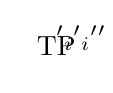
\begin{tikzpicture}[baseline=(root.base)]
    \Tree 	[.\node(root){TP};
                [.TP
                    {Cop$'$\\{is e$_{i}$}}
                    [.CopP
                        oileanach
                        {Cop$'$\\\tuple{is e}}
                    ]
                ]
                [.CP$_{i}$
                    a
                    [.FinP
                        tha
                        [.TP
                            pro
                            [.T$'$
                                \tuple{tha}
                                [.PredP
                                    \tuple{pro}
                                    [.Pred$'$
                                        Pred
                                        [.PP
                                            {ann an}
                                            {DP\\Calum}
                                        ]
                                    ]
                                ]
                            ]
                        ]
                    ]
                ]
            ]

\end{tikzpicture}
%\begin{forest}
%[TP [TP [Cop'\\{is e$_{i}$} ] [CopP [ oileanach ] [Cop'\\\tuple{is e} ] ] ] [CP$_{i}$  [ a ] [FinP [ tha ] [TP [ pro ] [T' \tuple{tha} [PredP [ \tuple{pro} ] [Pred' [ Pred ] [PP [ {ann an} ] [DP\\Calum ] ] ] ] ] ] ] ] ]
%\end{forest}
\end{figure}

Here the relative clause\is{relative clauses} \emph{a th'ann an Calum} abstracts over the property
variable denoted by the pro in the specifier of TP, giving the meaning of
the relative clause\is{relative clauses} as a set of properties which are properties of Calum. The
pronoun in the copular\is{copulas} clause gets its meaning by straightforward substitution,
and the copula\is{copulas} asserts that the property of studenthood is in the set of
properties that Calum has. This analysis simply extends the analysis of clefts
I offered in \citep{Adger2011b} to these characterising
\isi{clefts}.

The final question is, for this kind of reading, why the cleft\is{clefts} is
obligatory.  The answer to this, from the perspective outlined here, is simply
that the Qual function would otherwise apply to the subject of the clause. It
may be that this function is itself connected to some syntactic position (for
example, perhaps Qual can only apply to case marked DPs, and A-bar bound pro
does not have to be case marked because of its lack of overt morphology), but I
leave this question open here.

\section{Conclusion}

A standard view of predicate nominals (e.g.
\citealt{partee:87,Higginbotham:1987}) is that some projection of the nominal
has a predicative type (\tuple{e, t}) and that this is what is seen in apparent
examples of NP \isi{predication}. In developments of such theories, we see
three ``layers'' of projection in the DP (e.g. \citealt{zamparelli}): a kind
level, a predicative level, and an argumental level. The predicative level is
that used in cases of NP \isi{predication}.

However, this is clearly not the case in Gaelic, and the question is why?

One possibility is that Gaelic lacks the predicative projection of the nominal.
It has only a property level projection, and an argument level projection (this
is the view taken in \citealt{adger-ramchand:03}). But this is stipulative. The
alternative I suggest is that subjects of \isi{predication} in syntactic specifier
positions are generally impossible in nominals, as such subjects require
eventive functional structure to be introduced. The category N creates
predicates of individuals, not events, and the extended projection of N
develops the semantics of an individual, not of a state of affairs. This set of
constraints on the syntax--semantics interface leaves languages with a problem:
how do they build the meaning of NP predication? Gaelic shows us two ways in
which a language can solve this problem. The p-strategy involves co-opting
structure which does have an event variable, while the cleft-strategy uses a
relative clause to create the necessary semantic glue.

What of languages like English? Nominal \isi{predication} is restricted in such
languages too, when the presence of the verb \emph{be} is controlled for.
Nominals are decidedly odd in \emph{be}-less \isi{predication} compared to PPs
and APs:

\ea
    \ea With Lilly ?(being) a small cat, she can squeeze through the hole.
    \ex With Lilly sick, we should get some special cat food.
    \ex With Lilly under anaesthetic, we can go ahead with the operation
    \z
\z
From the perspective of the theory offered in this paper, English \emph{be} is
performing a function similar to, but more general than, Gaelic \emph{ann an}.
Indeed, even with \emph{be}, we can see the same restriction we found in
Gaelic, where, when the predicate is restricted to be an interval state by
using a temporal modifier, relative clause\is{relative clauses} modification becomes impossible:

\ea[?*]{Calum was a student for three years that Ian knew.}
\z
The same core principles regulating the relationship between syntax and
se\-man\-tics are at work in both kinds of languages, but they evade the
restrictions imposed by those principles in different ways.

%
%\section{Introduction}
%Phasellus maximus erat ligula, accumsan rutrum augue facilisis in. Proin sit amet pharetra nunc, sed maximus erat. Duis egestas mi eget purus venenatis vulputate vel quis nunc. Nullam volutpat facilisis tortor, vitae semper ligula dapibus sit amet. Suspendisse fringilla, quam sed laoreet maximus, ex ex placerat ipsum, porta ultrices mi risus et lectus. Maecenas vitae mauris condimentum justo fringilla sollicitudin. Fusce nec interdum ante. Curabitur tempus dui et orci convallis molestie \citep{Chomsky1957}.
%\citep{Comrie1981}
%
%\ea
%\gll dit          is           een             voorbeeld.\\
%     \textsc{dem} \textsc{cop} \textsc{indef}  example\\
%\glt \enquote*{This is an example.}
%\z
%
%
%Sed nisi urna, dignissim sit amet posuere ut, luctus ac lectus. Fusce vel ornare nibh. Nullam non sapien in tortor hendrerit suscipit. Etiam sollicitudin nibh ligula. Praesent dictum gravida est eget maximus. Integer in felis id diam sodales accumsan at at turpis. Maecenas dignissim purus non libero scelerisque porttitor. Integer porttitor mauris ac nisi iaculis molestie. Sed nec imperdiet orci. Suspendisse sed fringilla elit, non varius elit. Sed varius nisi magna, at efficitur orci consectetur a. Cras consequat mi dui, et cursus lacus vehicula vitae. Pellentesque sit amet justo sed lectus luctus vehicula. Suspendisse placerat augue eget felis sagittis placerat.
%
%
%\begin{table}
%\caption{Frequencies of word classes}
%\label{tab:1:frequencies}
% \begin{tabular}{lllll}
%  \lsptoprule
%            & nouns & verbs & adjectives & adverbs\\
%  \midrule
%  absolute  &   12 &    34  &    23     & 13\\
%  relative  &   3.1 &   8.9 &    5.7    & 3.2\\
%  \lspbottomrule
% \end{tabular}
%\end{table}
%
%
%Sed cursus eros condimentum mi consectetur, ac consectetur sapien pulvinar. Sed consequat, magna eu scelerisque laoreet, ante erat tristique justo, nec cursus eros diam eu nisl. Vestibulum non arcu tellus. Nunc dignissim tristique massa ut gravida. Nullam auctor orci gravida tellus egestas, vitae pharetra nisl porttitor. Pellentesque turpis nulla, venenatis id porttitor non, volutpat ut leo. Etiam hendrerit scelerisque luctus. Nam sed egestas est. Suspendisse potenti. Nunc vestibulum nec odio non laoreet. Proin lacinia nulla lectus, eu vehicula erat vehicula sed.



\printchapterglossary{}

\section*{Acknowledgements}

One of my first grown-up conference papers was at a Celtic syntax workshop
organised by Ian Roberts and Bob Borsley in Bangor. That paper argued that
measure phrases in \ili{Scottish Gaelic} were a kind of defective nominal, and
because of this defectiveness, they are incorporated into the syntactic and
semantic dependencies set up by the verbal extended projection. This paper
written in appreciation of Ian's important impact on my linguistic thinking
returns to that exact same intuition for predicate nominals, showing either
that I'm stubborn, or can't move on! I've presented this set of ideas at the
workshop on predication in Ontario, 2009,  then, after a long hiatus, at the
Universit\'e de Paris VIII in 2014 and at the University of Ulster in 2015. Many
thanks to all for comments and suggestions as well as to Caroline Heycock for
comments on an early version. Many thanks also to Iseabail NicIlleathain and
S\`ileas NicLe\`oid for help with data, to Jason Ostrove for checking some
examples for me while he was in the field, and to two anonymous reviewers for
this volume.

{\sloppy
\printbibliography[heading=subbibliography,notkeyword=this]
}

\end{document}
